\section{Basic}
\inputcodenohash{Shell Script}{Basic/Script.sh}
% \inputcode{Default Code}{Basic/DefaultCode.cpp}
% \inputcode{Increase Stack Size}{Basic/IncreaseStackSize.cpp}
\inputcode{Debug Macro}{Basic/DebugMacro.cpp}
\inputcodenohash{Pragma / FastIO}{Basic/Fast.cpp}
\inputcodenohash{Divide}{Basic/Div.cpp}

\section{Data Structure}
\inputcode{Leftist Tree}{DataStructure/LeftistTree.cpp}
\inputcode{Splay Tree}{DataStructure/Splay.cpp}
\inputcode{Link Cut Tree}{DataStructure/LinkCutTree.cpp}
\inputcode{Treap}{DataStructure/Treap.cpp}
% \inputcode{2D Segment Tree}{DataStructure/2DSeg.cpp} % Stress Test with Brute Force
\inputcode{vEB Tree}{DataStructure/vEBTree.cpp} % Library Checker "Predecessor Problem"
% \inputcode{Range Set}{DataStructure/RangeSet.cpp} % CF 981G, ABC 255H

\section{Flow / Matching}
\inputcode{Dinic}{FlowMatching/Dinic.cpp} % CSES
\inputcode{Min Cost Max Flow}{FlowMatching/MCMF.cpp} % CSES
\inputcode{Kuhn Munkres}{FlowMatching/KM.cpp} % TIOJ 2197
\inputcode{Hopcroft Karp}{FlowMatching/HopcroftKarp.cpp} % Library Checker "Matching on Bipartite Graph"
\inputcode{SW Min Cut}{FlowMatching/SW.cpp} % NTUJ 1878 (But NTUJ is broken now :/)
\inputcode{Gomory Hu Tree}{FlowMatching/GomoryHu.cpp} % CF 343E
\inputcode{Blossom}{FlowMatching/GeneralGraphMatching.cpp} % Library Checker "Matching on General Graph"
\inputcode{Min Cost Circulation}{FlowMatching/MinCostCirculation.cpp} % copy from 8BQube, (X) change style
\inputcode{Weighted Blossom}{FlowMatching/WeightGeneralGraphMatching.cpp} % Library Checker "General Weighted Matching", (X) change style
\inputtex{Flow Model}{FlowMatching/FlowModel.tex}

\section{Graph}
% \inputcode{Binary Lifting*}{Graph/BinaryLifting.cpp}
\inputcode{Heavy-Light Decomposition}{Graph/HeavyLightDecomp.cpp} % CSES
\inputcode{Centroid Decomposition}{Graph/CentroidDecomp.cpp} % CF 321C
\inputcode{Edge BCC}{Graph/EdgeBCC.cpp} % CF 1000E, Library Checker
\inputcode{Vertex BCC / Round Square Tree}{Graph/RoundSquareTree.cpp} % CF 962F, Library Checker
\inputcode{SCC}{Graph/SCC.cpp} % Library Checker
\inputcode{2SAT}{Graph/2SAT.cpp} % CF 1657F, Library Checker
\inputcode{Virtual Tree}{Graph/VirtualTree.cpp} % ABC 359G
\inputcode{Directed MST}{Graph/DirectedMST.cpp} % Almost Copy from ckiseki, CF 100307D, Library Checker
\inputcode{Dominator Tree}{Graph/DominatorTree.cpp} % Library Checker
\inputcode{Bipartite Edge Coloring}{Graph/BipartiteEdgeColoring.cpp} % CF 600F
\inputcode{Edge Coloring}{Graph/Vizing.cpp}
\inputcode{Maximum Clique}{Graph/MaxCliqueDyn.cpp} % Library Checker, (X) change style

\section{String}
\inputcode{Aho–Corasick Automaton}{String/AC.cpp}
\inputcode{KMP Algorithm}{String/KMP.cpp}
\inputcode{Z Algorithm}{String/Z.cpp} % Library Checker
\inputcode{Manacher}{String/Manacher.cpp} % Library Checker
\inputcode{Suffix Array}{String/SA.cpp} % Library Checker
\inputcode{SAIS}{String/SAIS.cpp} % Library Checker
\inputcode{Suffix Automaton}{String/SAM.cpp}
\inputcode{Minimum Rotation}{String/MinRotation.cpp} % NTUJ 1751
\inputcode{Palindrome Tree}{String/PalindromeTree.cpp}
\inputcode{Lyndon Factorization}{String/LyndonFactorization.cpp} % Copy from ckiseki
\inputcode{Main Lorentz}{String/MainLorentz.cpp} % CF 1043G, Library Checker

\section{Math}
% \inputcode{Fraction*}{Math/Fraction.cpp}
\inputcode{Miller Rabin / Pollard Rho}{Math/MillerRabinPollardRho.cpp} % Library Checker
\inputcode{Ext GCD}{Math/Extgcd.cpp} % Stress Tests
\inputcode{Chinese Remainder Theorem}{Math/CRT.cpp} % ABC 193E
\inputcode{PiCount}{Math/PiCount.cpp} % Library Checker
\inputcode{Linear Function Mod Min}{Math/LinearFuncModMin.cpp} % Library Checker
% \inputcode{Determinant}{Math/Determinant.cpp} % Library Checker
\inputcode{Floor Sum}{Math/FloorSum.cpp} % ABC 313G, Library Checker
\inputcode{Quadratic Residue}{Math/QuadraticResidue.cpp} % Library Checker
\inputcode{Discrete Log}{Math/DiscreteLog.cpp} % Library Checker
\inputcode{Factorial without Prime Factor}{Math/FacNoP.cpp} % From 8BQube
\inputcode{Berlekamp Massey}{Math/BerlekampMassey.cpp} % Library Checker
\inputcode{Simplex}{Math/Simplex.cpp} % CF 101161J
\inputtex{Euclidean}{Math/Euclidean.tex}
\inputtex{Linear Programming Construction}{Math/LPConstruction.tex}
\inputtex{Theorem}{Math/Theorem.tex}
\inputtex{Estimation}{Math/Estimation.tex}
\inputtex{General Purpose Numbers}{Math/number.tex}
% \inputtex{Tips for Generating Funtion*}{Math/gf.tex}

\section{Polynomial}
\inputcode{Number Theoretic Transform}{Polynomial/NTT.cpp}
\inputcode{Fast Fourier Transform}{Polynomial/FFT.cpp}
\inputtex{Primes}{Polynomial/NTTprime.tex}
\inputcode{Polynomial Operations}{Polynomial/Operation.cpp}
\inputcode{Fast Linear Recursion}{Polynomial/FastLinearRecursion.cpp}
\inputcodenohash{Fast Walsh Transform}{Polynomial/Fwt.cpp}

\section{Geometry}
\inputcodenohash{Basic}{Geometry/BasicSimple.cpp}
\inputcodenohash{SVG Writer}{Geometry/SVGWriter.cpp}
\inputcode{Heart}{Geometry/Heart.cpp}
\inputcode{External Bisector}{Geometry/External_bisector.cpp}
\inputcode{Intersection of Segments}{Geometry/Intersection_of_Segments.cpp}
\inputcode{Intersection of Circle and Line}{Geometry/Intersection_of_Circle_and_Line.cpp}
\inputcode{Intersection of Circles}{Geometry/Intersection_of_Circles.cpp}
\inputcode{Intersection of Polygon and Circle}{Geometry/Intersection_of_Polygon_and_Circle.cpp}
\inputcode{Tangent Lines of Polygon and Point}{Geometry/Tangent_Lines_of_Polygon_and_Point.cpp}
\inputcode{Tangent Lines of Circle and Point}{Geometry/Tangent_Lines_of_Circle_and_Point.cpp}
\inputcode{Tangent Lines of Circles}{Geometry/Tangent_Lines_of_Circles.cpp}
\inputcode{Point In Convex}{Geometry/PointInConvex.cpp} % ABC 296G
\inputcode{Point In Circle}{Geometry/PointInCC.cpp}
\inputcode{Point Segment Distance}{Geometry/PointSegDist.cpp}
\inputcode{Convex Hull}{Geometry/ConvexHull.cpp}
% \inputcode{Convex Hull Distance}{Geometry/ConvexHullDist.cpp}
\inputcode{Minimum Enclosing Circle}{Geometry/Minimum_Enclosing_Circle.cpp}
\inputcode{Union of Circles}{Geometry/Union_of_Circles.cpp} % TIOJ 1503
\inputcode{Union of Polygons}{Geometry/Union_of_Polygons.cpp} % CF 107E, CF 101673A
% \inputcode{Rotating Caliper}{Geometry/RotatingCaliper.cpp}
\inputcode{Rotating SweepLine}{Geometry/RotatingSweepLine.cpp}
\inputcode{Half Plane Intersection}{Geometry/HalfPlaneIntersection.cpp} % Kattis Big Brother
\inputcode{Minkowski Sum}{Geometry/MinkowskiSum_Linear.cpp} % CF 1841F
\inputcode{Vector In Polygon}{Geometry/VectorInPoly.cpp} % Yokohama 2022 Regional pJ
\inputcode{Delaunay Triangulation}{Geometry/DelaunayTriangulation.cpp} % NTUJ 3667, CF acmsgrur 383
\inputcode{Triangulation Vonoroi}{Geometry/Triangulation_Vonoroi.cpp} % NTUJ 3667, CF acmsguru 383
\inputcodenohash{3D Point}{Geometry/3DPoint.cpp}
\inputcode{3D Convex Hull}{Geometry/3DConvexHull.cpp}

\section{Else}
\inputcodenohash{Pbds}{Else/Magic.cpp}
\inputcodenohash{Bit Hack}{Else/BitHack.cpp}
% \inputtex{Dynamic Programming Condition}{Else/Condition.tex}
\inputcode{Smawk Algorithm}{Else/Smawk.cpp}
\inputcode{Slope Trick}{Else/SlopeTrick.cpp}
% \inputcode{Manhattan MST}{Else/ManhattanMST.cpp}
% \inputcode{Dynamic MST}{Else/DynamicMST.cpp}
\inputcode{ALL LCS}{Else/All_LCS.cpp}
\inputcode{Hilbert Curve}{Else/Hilbert.cpp}
% \inputcodenohash{Random}{Else/Random.cpp}
\inputcode{Line Container}{Else/LineContainer.cpp}
\inputcode{Min Plus Convolution}{Else/MinPlusConvolution.cpp}
\inputtex{Matroid Intersection}{Else/Matroid.tex}
\inputcodenohash{Simulated Annealing}{Else/SimulatedAnnealing.cpp}
\inputcodenohash{Bitset LCS}{Else/BitsetLCS.cpp}
\inputcode{Binary Search On Fraction}{Else/BinarySearchOnFraction.cpp}
\inputcode{Cyclic Ternary Search}{Else/CycTsearch.cpp}
\inputcode{Tree Hash}{Else/TreeHash.cpp}
\inputcodenohash{Python Misc}{Else/python.py}
% \includegraphics[scale=0.38]{Else/Convex.png}
\begin{center}
    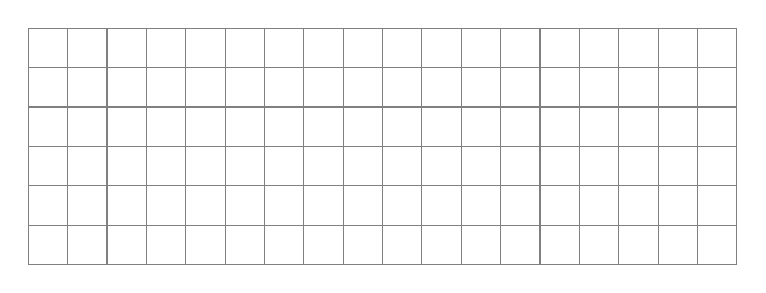
\begin{tikzpicture}
        \draw[step=0.5, gray, thin] (0,0) grid (9.0, 3);
    \end{tikzpicture}
\end{center}